%!TEX root = ../thesis.tex
\section{実験2 提案手法による人追従の実験}

\subsection{実験目的}
\subsection{実験方法}

  \begin{figure}[h]
    \centering
    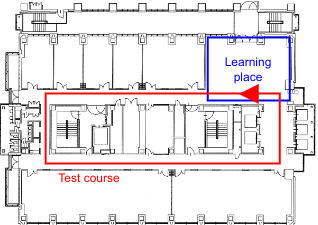
\includegraphics[keepaspectratio, scale=0.80] {images/RobotGuidance_course.png}
    \captionsetup{justification=raggedright} % キャプションを左寄せに
    \caption{Learning and following phase courses}
    \label{Fig:RobotGuidance_course}
  \end{figure}

\subsection{結果と考察}

  \begin{figure}[h]
    \centering
    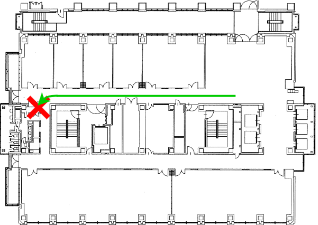
\includegraphics[keepaspectratio, scale=0.80] {images/RobotGuidance_failed_experiment.png}
    \captionsetup{justification=raggedright} % キャプションを左寄せに
    \caption{Failed at the first corner}
    \label{Fig:RobotGuidance_failed_experiment}
  \end{figure}

  \begin{figure}[h]
    \centering
    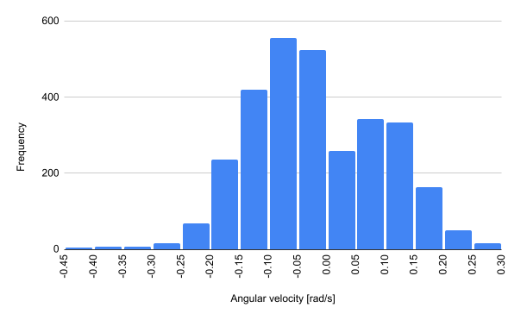
\includegraphics[keepaspectratio, scale=0.60] {images/RobotGuidance_failed_histogram.png}
    \captionsetup{justification=raggedright} % キャプションを左寄せに
    \caption{Histogram of angular velocity at failure}
    \label{Fig:RobotGuidance_failed_histogram}
  \end{figure}

\newpage
